\section{Implementation and experiments}\label{sec:exp}
% =====================================================================
% Section 7: Implementation and experiments
% Sources (final records only):
%   research/tracks/experiments/notes-final.md (v2): sections 0-6, Props E1-lit, E1-pf, E1-al, E2, E3, Thm E4,
%     Props E4-share, E5, E6, E7, Lemma E8.1, Prop E8, Cors E8.2, E8.3, Prop E9, Prop E10, Lemma V, and the
%     verification log (section 8); research/tracks/experiments/referee.md (F1-F8, R1-R17).
%   code/README.md and code/results/*.md (every number below was checked against these files);
%     code/experiments/recheck/*.out (referee's oracle checks re-run against v2).
%   research/prior/induction/second-order-notes.md (C3, C9) and research/prior/pa-untagged/ for the prior results
%     that E2 and E6 reproduce.
% =====================================================================

This section describes an implementation of the determinate-template learner and of \DTRC{}, and the experiments run with it. The implementation answers two needs. It checks the theory of \cref{sec:single,sec:univ,sec:zf,sec:many} on data that the theory did not choose. And it shows what goes wrong in practice when the hypotheses of those theorems fail: when the refutation search has a budget, when targets look alike, and when the data contain mistakes. The package \texttt{dtrc} (pure Python, in \texttt{axiom-schemas/code/}) was written by the experiments track and is independent of the untagged track's prototype used in \cref{sec:many}. An adversarial referee re-ran every experiment, wrote independent checks, and found one false claim and one false proposition in the first version of the record; both are corrected below and listed in \cref{app:ver}.

Status markers are as elsewhere; \emph{computed} means that a script was run and its output is in \texttt{code/results/} (commands in \cref{app:exp:repro}). Every random choice is seeded. Re-running reproduces every number except timings exactly. Full proofs are in \cref{app:exp}.

\paragraph{Findings in brief.}
\begin{itemize}
\item \emph{Q1} (\cref{sec:univ}). The implemented learner and the first-order $\lgg$ both learn the instance schema, and they become exact at the same $N$ in every run; the mean number of instances matches the head-variation prediction.
\item \emph{Q2} (\cref{sec:zf}). The learner is exact on Separation, Replacement ($\exists!$ spelled out) and $\in$-induction from $2$--$3$ instances, and on PA induction, with no non-instance accepted in 927 probes. A genuine pattern $\lgg$ is also exact on the three ZF schemas and never on induction. First-order $\lgg$s are unsound except on $\in$-induction in de Bruijn indices.
\item \emph{Q3} (\cref{sec:many}). On untagged mixtures of the PA and ZF axioms and schemas, \DTRC{} recovers the hidden labels in every run and accepts no non-target probe. With a sharing pass for ambiguous data it is exactly as good as the tagged learner given every label a datum deserves. We prove that the mixtures satisfy refutation separation; the experiments' evidence for separation is narrow beyond them.
\item \emph{Failures.} With injected mistakes and a refutation budget of $80$ or $400$ instances, \DTRC{} \emph{accepted a false sentence} (budget $2000$ removed it). Similar targets can merge into valid templates that no world-based refutation can separate. Positive-arity term metavariables make the minimal covering sets blow up.
\end{itemize}

% ---------------------------------------------------------------------
\subsection{What was implemented}\label{sec:exp:impl}

\paragraph{Data.}
Terms and formulas are trees with de Bruijn indices for bound variables and named parameters, over $L_A$ and $L_\in$ (\cref{sec:setting}). A datum is in closure-normal form, and each datum is canonicalized on its own: its parameters are renamed $w_0,w_1,\dots$ in order of first occurrence. Leading universal quantifiers are \emph{not} stripped. So the axiom Q4 is the datum $\forall x\,(x+0=x)$, and $w_0+0=w_0$ is a different datum for the same proposition; the schema $z+0=z$ accepts the second, not the first. With this choice the targets of the PA mixture below have pairwise disjoint instance sets except for the one sentence $0+0=0$, which instantiates both $z+0=z$ and $0+z=z$, and the targets of the ZF mixture are pairwise disjoint (the proof of \cref{prop:exp:mixsep} exhibits a rigid clash for every pair). Under full stripping (leading $\forall$ replaced by fresh parameters) Q4 would be an instance of $z+0=z$ and Q6 of $z\cdot0=0$. The referee re-ran \DTRC{} with all data and targets stripped: labels were still recovered (ARI $1$ on unambiguous data), Q4 and Q6 were absorbed into the clusters of $z+0=z$ and $z\cdot0=0$, and no non-target probe was accepted \src{experiments \S1.1; referee R13}.

Because data are canonicalized one by one, the matcher decides membership \emph{up to an injective renaming of the template's parameters}. In this section $\inst(T)$, ``covers'' and $\gen$ are read in this sense ($\inst^{\sim}$ and $\gen^{\sim}$ of \cref{app:setting}); for parameter-free templates nothing changes. Anchors are taken in the class $\{\inst(T):T\in\DTF\}$.

\paragraph{The class $\DTF$.}
The implemented class is $\DTF$: determinate templates whose term metavariables are $0$-ary; formula metavariables keep any arity (\cref{sec:setting}). Three reasons. (1)~Every target used below lies in $\DTF$: $\Q$'s axioms, $T_{\Ind}$, the instance schemas, all ZF axioms and schemas, and all near-miss and hard targets. A target in the class is closed in the class, so the cautious verifier stays sound (\cref{sec:setting}). (2)~Positive-arity term metavariables blow up the minimal covering sets (experiment E7 below). In $L_\in$ a term metavariable $f(\bar y)$ can only denote a projection or a parameter, and any variable column can be derived from any other. (3)~Since $\DTF\subseteq\DT$, every anchor in $\DT$ is an anchor in $\DTF$; the classes differ only before an anchor. For example, $\{\Ind(x=x),\Ind(0=x)\}$ has $4$ minimal covering templates in $\DT$ and $2$ in $\DTF$ \src{experiments \S2.1}.

\paragraph{Minimal covering templates.}
The learner needs $\Min_F(D)$, the minimal covering templates of $D$ in $\DTF$ up to parameter renaming. It computes them from a finite normal form. Let $C(D)$ be the \emph{common-prefix tree} of $D$: the positions at which all data carry the same label and arity (parameters compared by name), together with the \emph{slots}, the maximal positions at which the data disagree. The \emph{column} at a position $p$ is $(d|_p)_{d\in D}$; it is \emph{open} if some $d|_p$ has a free index, i.e.\ a variable bound above $p$. In $\mathcal T(D)$ every common atom node whose subtree contains a slot with an open column is cut to a leaf slot, an \emph{F-slot}; so every term slot of $\mathcal T(D)$ has a closed column.

\begin{definition}[Normal configurations]\status{definition}\src{experiments \S1.3}\label{def:exp:normal}
For a slot $\sigma$ of $\mathcal T(D)$ let $\bar y_\sigma$ list the free indices of its column, let $M_\sigma$ be a fresh metavariable of the slot's sort and arity $|\bar y_\sigma|$, and let $\beta_d(\sigma)$ be $d|_\sigma$ abstracted over $\bar y_\sigma$. A node $\pi$ of $\mathcal T(D)$ is \emph{derivable} from $\sigma$, $\sigma\to\pi$, if there are metavariable-free terms $\bar t$ with $\beta_d(\sigma)[\bar t]=d|_\pi$ for all $d\in D$; then $\bar t=:\bar t(\sigma,\pi)$ is unique. A \emph{normal configuration} consists of a set $S'$ of slots, none derivable from another; an antichain $A\supseteq S'$ of nodes of $\mathcal T(D)$ such that every slot lies at or below a member of $A$; and a choice of $c(\pi)\in S'$ with $c(\pi)\to\pi$ for each $\pi\in A\setminus S'$. Its template carries $M_\sigma(\bar y_\sigma)$ at $\sigma\in S'$, $M_{c(\pi)}(\bar t(c(\pi),\pi))$ at $\pi\in A\setminus S'$, and the common labels elsewhere.
\end{definition}

\begin{proposition}[Normal form]\status{proved; computed}\src{experiments Props E1-lit, E1-al; E0, E0b}\label{prop:exp:normal}
Let $D$ be finite and nonempty, with parameters compared by name.
\textup{(a)} Every normal configuration lies in $\DTF$ and covers $D$.
\textup{(b)} Every $T\in\DTF$ that covers $D$ satisfies $T\gen N$ for some normal configuration $N$.
\textup{(c)} Hence the $\gen$-minimal normal configurations form a finite set $\Min^{\mathrm{lit}}_F(D)$; every covering $T\in\DTF$ lies above a member; members are minimal among all covering templates in $\DTF$; and if $D\subseteq\inst(T^*)$ with $T^*\in\DTF$, some member lies below $T^*$.
\end{proposition}

\begin{proof}[Proof idea]
(a) is a direct check. For (b), let $T$ cover $D$. Rigid symbols of $T$ survive instantiation, so the skeleton of $T$ lies in $C(D)$, and an occurrence cannot sit strictly below an F-slot (a $0$-ary term metavariable inside an atom has a closed value, while the F-slot contains an open column). Push each pattern occurrence that sits above a slot down through the common labels, drop argument places that no datum uses, observe that the remaining arguments are forced, and finally replace an own slot that is derivable from another by the derived occurrence. Each step specializes $T$ and keeps it covering; the result is a normal configuration. Full proof in \cref{app:exp:normal}.
\end{proof}

With parameters compared up to renaming, $\Min_F(D)$ is the set of minimal elements of the union of $\Min^{\mathrm{lit}}_F(\alpha(D))$ over all \emph{alignments} $\alpha$ of the data's parameters, as defined in \cref{app:setting}; \cref{prop:exp:normal}(c) supplies the finiteness property used there, so (a)--(c) hold for $\Min_F(D)$ with $\gen^{\sim}$ (the alignment proposition of \cref{app:setting}). Literal comparison is not enough: the first version of the record stated (c) for renaming-closed covering, and the referee found a counterexample with a rigid parameter (\cref{app:setting}). The code enumerates normal configurations, filters them by generality (decided by matching frozen templates, \cref{sec:setting}), caps the number of alignments at $4096$ and reports truncation; no truncation occurred in any experiment. If some datum has no parameter there is one alignment. On the experiment data the two sets rarely differ: in $0$ of the $720$ data sets of E2, and in one $\Min$ call over all \DTRC{} runs of E3 \src{experiments \S3.1, E2, E3}.

Two computed checks back the normal form. E0 compares the code with the prior referee's bounded enumerator on 48 arithmetic data sets ($3703$ covering $\DTF$ templates of size $\le14$, $2515$ $\DT$ templates of size $\le13$): no enumerated template fails to lie above a computed minimum, and none lies strictly below one. Its coverage is narrow (no ${<}$, ${\in}$, ${\leftrightarrow}$ or parameters; 41 of the 48 sets have $|\Min|=1$). E0b uses the referee's random template generator in both languages, with and without a rigid parameter, $200$ data sets per cell: the alignment-complete $\Min_F$ has no failure in any cell, while the literal set misses the generating template in $17/200$ (PA) and $36/200$ (ZF) data sets with a rigid parameter and in none without (\cref{app:exp:normal}).

\paragraph{World oracles.}
Two three-valued evaluators return True, False, or unknown. \emph{PA} (truth in $\N$): numerals are evaluated exactly; atoms with symbolic variables are decided by polynomial normal forms over $\N$; bounded quantifiers with numeral bounds are enumerated; numeral search finds counterexamples and witnesses; and, in the revised version, an unbounded quantifier is case-split into $x\in\{0,1\}$ and $x=x'+2$ with $x'$ fresh. \emph{ZF} (truth in $V$): hereditarily finite sets of rank $\le3$ plus \emph{generic objects}; for an unbounded quantifier the universe is split into three cases, $x$ in the transitive closure $E$ of the concrete values in scope, $x$ equal to a generic in scope, or $x$ a fresh generic. Both use Kleene's strong three-valued connectives \citep{kleene1952introduction} with supervaluation over the unknown leaves \citep{vanfraassen1966singular}, and both first simplify by \emph{constant propagation}: propositional laws valid in every nonempty structure, after replacing by $\top$ or $\bot$ the atoms whose value does not depend on the variables ($t=t$; closed arithmetic atoms; $t<t$ in $\N$; $x\in x$ in $V$, by Foundation).

\begin{proposition}[The oracles are sound]\status{proved; computed}\src{experiments Prop E2; recheck R3, R4, R11}\label{prop:exp:oracle}
If the PA evaluator returns True (False) on a datum, its universal closure is true (false) in $\N$. Assume $V\models\ZF$. If the ZF evaluator returns True (False) on a datum, its universal closure is true (false) in $V$.
\end{proposition}

\begin{proof}[Proof idea]
Induction on the formula, for a fixed environment of concrete values and generics, with the claim for the ZF evaluator made for every \emph{realization} of the generics (each generic denotes a set outside the transitive closure $E$ fixed when it was introduced, distinct from the generics then in scope). The atom rules are sound: for instance, a generic $G$ is not an element of a concrete $c\subseteq E_G$, and $G\in G$ is false by Foundation. The three cases of an unbounded quantifier cover every set: a set outside $E$ that is not an in-scope generic is a legitimate value of a fresh generic. Kleene's tables are monotone, and supervaluation enumerates a superset of the realizable assignments to the unknown leaves. Full proof in \cref{app:exp:oracle}.
\end{proof}

The proof uses Foundation, Extensionality on HF sets, the existence of HF sets, and that no set contains all sets; it does not use Infinity. The referee's independent evaluators were re-run against the revised oracles: $0$ contradictions on $2197$ PA and $413+179$ ZF verdicts logged during \DTRC{} runs (the latter of quantifier depth $\le4$ and $5$--$6$), and on $3000$ random PA and $600$ random ZF sentences. The independent ZF check evaluates exactly in finite structures $V_4\cup\{\text{extra objects}\}$ that satisfy exactly the proof's assumptions; a mutation test shows it has power (dropping the in-scope-generic case is detected $39/600$ times, dropping the fresh-generic case $292/600$ times). Neither oracle is complete. The ZF evaluator cannot refute a sentence whose refutation needs a witness \emph{constructed} from a generic, such as $\forall a\exists b\forall x\,(x\in b\leftrightarrow a\in x)$; the PA evaluator leaves $\forall x\,(x=0\vee\exists y\,x=Sy)$ undecided. Both are truth oracles, not provability oracles \src{experiments \S3.2, \S5}.

\paragraph{The template refuter.}
A template is \emph{refuted} once the oracle returns False on one of its instances. The refuter searches instances under a budget (default $80$ instances), in this order: every $\top/\bot$ assignment to the formula metavariables; one metavariable running through a pool of small bodies while the others are $\top$ (or $\bot$); parallel and diagonal enumerations of small bodies per sort and arity; and bodies read off the data by matching. It is \emph{sound} (it reports only oracle refutations), \emph{budgeted}, and \emph{history-dependent}: it caches verdicts per template and accumulates data-guided tries across calls. It is therefore not a fixed oracle $\Ref_d$ in the sense of \cref{sec:setting}, and the guarantees below are stated for it directly. Every ``refuted'' count below is a lower bound on what an ideal refuter (one that refutes every template with a false instance) would refute, and ``not refuted'' is no evidence of truth.

\paragraph{\DTRC{} as implemented.}
(1)~Canonicalize the data and discard the data the oracle refutes. (2)~Agglomerate from singletons, trying pairs of clusters in decreasing order of common-prefix size; the merge of $A$ and $B$ succeeds iff some member of $\Min_F(A\cup B)$ is not refuted; a pair that failed stays failed for all clusters containing its parts. (3)~Optionally, a \emph{sharing pass}: for each final cluster $C$ and each kept datum $d\notin C$, in data order, add $d$ to $C$ if the merge test on $C\cup\{d\}$ succeeds; clusters may then overlap. (4)~For each cluster $C$, the cautious verifier with refutation: $\Acc(C)=\bigcap\{\inst(T):T\in\Min_F(C)\text{ not refuted}\}$, and $\Acc(C)=C$ if every member is refuted. (5)~Assert $\bigcup_C\Acc(C)$. This is $\DTRC$ of \cref{sec:many} with the class $\DTF$, a fixed merge order, a budgeted refuter, and the optional sharing pass.

\paragraph{Baselines and references.}
(i)~First-order $\lgg$ per tag \citep{plotkin1970note,reynolds1970transformational} in a named encoding (binders carry level names) and in de Bruijn indices; instantiation may capture, as first-order substitution permits. (ii)~Higher-order pattern $\lgg$ per tag: the common prefix with, at each slot, a fresh variable applied to the bound variables free in the slot's column, shared between slots whose columns agree up to a permutation of those variables (the track's reading of the merge rule of \citet{baumgartner2017higher}; their implementation was not run). The \emph{genuine} version generalizes a term disagreement that contains a bound variable by a term variable $f(x,\dots)$ of positive arity; it lies in $\DT$, not in $\DTF$. The \emph{formula-level} version, used in the first version of the record, generalizes the enclosing atom by a formula variable instead; on $\{\Sep(x\in a),\Sep(a\in x)\}$ it returns $T_{\Sep}$, while the genuine one returns the strictly more specific $\forall a\exists b\forall x\,(x\in b\leftrightarrow x\in a\wedge f(x,a)\in f(a,x))$. (iii)~The cautious $k$-union verifier over $\DTF$ (all partitions into at most $k$ blocks), with and without refutation negatives, for small cases. (iv)~\emph{Skeleton clustering}: \DTRC{} without refutation, stopped at the true number of targets. (v)~The tagged refutation-filtered verifier, given \emph{gold labels} (the target each datum was generated from) or \emph{membership labels} (every target the datum instantiates).

\paragraph{Datasets and metrics.}
\emph{PA-mix}: Q1--Q7 as closed sentences; $30$ induction instances with random motives (parameters allowed); and $8$, $6$, $4$ instances of $U_{\mathrm{add0}}=(z+0=z)$, $U_{\mathrm{mul0}}=(z\cdot0=0)$, $U_{\mathrm{0add}}=(0+z=z)$. In the main regime the universal axioms are seen only through numeral instances $n+0=n$, $n\cdot0=0$, $0+n=n$ with $n$ uniform in $0..7$ (we write numerals as digits). In the \emph{mixed} regime (the first version's) $z$ is a numeral with probability $0.6$, a random closed term of depth $\le2$ with probability $0.25$, and a parameter (the axiom in parameter form) with probability $0.15$. \emph{ZF-mix}: $\Ext,\Pair,\Union,\Pow,\Inf,\Found$; $12$ Separation, $10$ Replacement ($\ReplS$, $\exists!$ spelled out, image consequent) and $10$ $\in$-induction instances with random small bodies (bounded quantifiers and parameters allowed). \emph{Stress sets}: near-miss targets, injected mistakes, unequal frequencies, and a set of hard ZF pairs (E4, E9 below). \emph{Held-out sets} contain schema instances only and are disjoint from the training data.

Metrics. The adjusted Rand index (ARI; \citealp{hubert1985comparing}) of the clustering against the gold labels, on unambiguous data. \emph{Exactness}: a schema target counts as exact when its cluster (or tag) passes a sufficient syntactic test for $\Acc=\inst(T^*)$: every unrefuted minimal template is $\gen T^*$ and one of them is $\preceq T^*$. A ground axiom counts as exact when it stays a singleton cluster that accepts exactly the axiom; we report this separately, because it is trivial. \emph{Held-out acceptance}. \emph{Probes}: sampled accepted sentences, how many of them are instances of no target, and how many of those the oracle refutes. A probe count is a lower bound on unsoundness, never a certificate of truth-soundness (\cref{prop:exp:qF}).

% ---------------------------------------------------------------------
\subsection{Guarantees for the implemented learner}\label{sec:exp:theory}

The theorems of \cref{sec:many} are stated for a fixed oracle and the class $\DT$. The following statements are their analogues for $\DTF$, $\Min_F$ and the budgeted, history-dependent refuter. Throughout, the world is $\N$ or $V$ and the refuter is sound.

\begin{proposition}[Merge monotonicity; within-target merges succeed]\status{proved}\src{experiments Prop E3}\label{prop:exp:mono}
\textup{(a)} Let $D\subseteq D'$ and let the refuter be ideal. If every member of $\Min_F(D)$ is refuted, so is every member of $\Min_F(D')$.
\textup{(b)} If $X\subseteq\inst(T^*)$ with $T^*\in\DTF$ and every instance of $T^*$ is true, then the merge test on $X$ succeeds, for every sound refuter and budget.
\end{proposition}

\begin{proof}
(a) A member $T'$ of $\Min_F(D')$ covers $D$, so $T'\gen T$ for some $T\in\Min_F(D)$, and $T$'s false instance lies in $\inst(T')$. (b) Some $T_0\in\Min_F(X)$ satisfies $T_0\preceq T^*$ (\cref{prop:exp:normal}(c) with alignments). All its instances are true, so no sound refuter refutes it.
\end{proof}

\begin{theorem}[\DTRC{} under refutation separation]\status{proved}\src{experiments Thm E4}\label{thm:exp:dtrc}
Assume (T) targets $T_1,\dots,T_k\in\DTF$ all of whose instances are true; (D) data $D=D_1\sqcup\dots\sqcup D_k$ with $D_i\subseteq\inst(T_i)$, each datum an instance of exactly one target; (R) a sound refuter; and (S) every merge test on $A\cup B$ with $\emptyset\neq A\subseteq D_i$, $\emptyset\neq B\subseteq D_j$, $i\neq j$, fails, i.e.\ every member of $\Min_F(A\cup B)$ is refuted when the test examines it. Then \DTRC{} without the sharing pass discards no datum, and its final clusters are exactly the nonempty $D_i$. For each $i$, $\Acc(D_i)\subseteq\inst(T_i)$, so the asserted union is target-sound; and $\Acc(D_i)=\inst(T_i)$ whenever $D_i$ contains an anchor of $T_i$. If moreover \textup{(H-ref)} the refuter's verdict on a template does not depend on the call history, then $\Acc(D_i)$ is the acceptance set of the tagged refutation-filtered verifier on $D_i$.
\end{theorem}

\begin{proof}[Proof idea]
Genuine data are true and are not discarded. Every cluster stays inside one $D_i$: cross merges fail by (S), and within-label merges succeed by \cref{prop:exp:mono}(b). So failed pairs are cross-label, inheriting failure never blocks a within-label merge, and the agglomeration ends only when no two clusters share a label. In $D_i$ the never-refuted $T_0\preceq T_i$ of \cref{prop:exp:mono}(b) is one of the intersected templates, which gives soundness; with an anchor every covering template contains $\inst(T_i)$, which gives exactness. Details in \cref{app:exp:dtrc}.
\end{proof}

The first version of the record also claimed that the union contains $\inst(T_i)$ \emph{exactly} for those $i$ where the tagged learner is exact; the ``only if'' half fails when instance sets overlap, so exactness is stated per cluster. Without (H-ref) (the implemented refuter caches data-guided tries) the two learners can differ, and only soundness and anchor-exactness are guaranteed \src{experiments \S8, referee F8}. With an ideal refuter, (S) reduces to pairs of single data, by \cref{prop:exp:mono}(a) (\cref{cor:exp:mixsep}); \cref{sec:many} states the same reduction for its separation condition.

\begin{proposition}[Per-cluster soundness does not depend on the budget]\status{proved}\src{experiments Prop E5}\label{prop:exp:budget}
If a cluster $C$ satisfies $C\subseteq\inst(T^*)$ with $T^*\in\DTF$ and all instances of $T^*$ true, then $\Acc(C)\subseteq\inst(T^*)$ for every sound refuter; more refutations only enlarge $\Acc(C)$.
\end{proposition}

\begin{proof}
The template $T_0\preceq T^*$ of \cref{prop:exp:mono}(b) is never refuted, so it is intersected, and $\Acc(C)\subseteq\inst(T_0)\subseteq\inst(T^*)$. Removing members from an intersection enlarges it.
\end{proof}

So a budgeted refuter can harm \DTRC{} only through clustering: a merge across targets, or with a mistake, that the refuter does not refute. Such a mixed cluster is truth-sound if one of its unrefuted minimal templates is valid, and may accept false sentences otherwise (\cref{prop:exp:qF}).

\begin{proposition}[The sharing pass]\status{proved}\src{experiments Prop E4-share}\label{prop:exp:share}
Assume (T) and (R), data $D\subseteq\bigcup_l\inst(T_l)$ (a datum may instantiate several targets), and:
(S$^+$) every merge or sharing test on a set $X\subseteq D$ contained in no $\inst(T_l)$ fails; and
(P) every final cluster $C$ of the agglomeration phase is contained in exactly one $\inst(T_l)$, written $T_{l(C)}$.
Then $l$ is injective on these clusters; after the sharing pass the cluster of target $l$ is $C^+=D\cap\inst(T_l)$, whatever the order; and $\Acc(C^+)\subseteq\inst(T_l)$, with equality whenever $D\cap\inst(T_l)$ contains an anchor of $T_l$. Under \textup{(H-ref)}, $\Acc(C^+)$ is the acceptance set of the tagged learner with membership labels.
\end{proposition}

The proof is in \cref{app:exp:dtrc}. The pass matters for the numerals regime. There $0+0=0$ is the only datum whose substituted term has head $0$ for both $U_{\mathrm{add0}}$ and $U_{\mathrm{0add}}$, so it is the only possible anchor of either (\cref{prop:exp:numerals}), and a partition gives it to at most one of them.

\begin{proposition}[Anchors of one-variable instance schemas in $\DTF$]\status{proved; computed}\src{experiments Prop E7; referee R2}\label{prop:exp:numerals}
Let $T^*$ contain one $0$-ary term metavariable $z$, at rigid positions, and no other metavariable and no parameter, and let $D\subseteq\inst(T^*)$ contain a parameter-free datum. Then $\Min_F(D)=\{T^*\}$ iff the terms substituted for $z$ do not all have the same root symbol ($0$ and each parameter count as root symbols). Hence for i.i.d.\ terms with root law $(p_h)_h$, $\Pr[\text{not exact after }N]=\sum_hp_h^N$; for numerals uniform in $0..7$ a sample is an anchor iff it contains the instance at $0$.
\end{proposition}

This is the anchor criterion of \cref{sec:univ} (Plotkin's \evR) for the implemented class; the proof is in \cref{app:exp:dtrc}. The referee found $0$ violations in $3000$ random data sets over $9$ one-variable templates.

\paragraph{Separation of the mixtures.}
The refutation-separation hypothesis (S) is a property of the run. For the targets of the two mixtures it can be proved outright, for an ideal refuter, by a case analysis of the minimal templates of cross pairs.

\begin{proposition}[Pairwise separation of the mixture targets]\status{proved; computed}\src{experiments Prop E8; E10}\label{prop:exp:mixsep}
Let $T_i\neq T_j$ both be PA-mix targets (Q1--Q7, $T_{\Ind}$, $U_{\mathrm{add0}}$, $U_{\mathrm{mul0}}$, $U_{\mathrm{0add}}$) or both ZF-mix targets ($\Ext$, $\Pair$, $\Union$, $\Pow$, $\Inf$, $\Found$, $T_{\Sep}$, $\ReplS$, $T_{\EInd}$), and let $a\in\inst(T_i)\setminus\inst(T_j)$, $b\in\inst(T_j)\setminus\inst(T_i)$. Then every member of $\Min_F(\{a,b\})$ has the form shown in \cref{tab:exp:cases}, with the false instance shown.
\end{proposition}

\begin{table}[t]
\centering\small
\begin{tabularx}{\textwidth}{@{}l>{\raggedright\arraybackslash}Xll@{}}
\toprule
case & target pairs & members of $\Min_F(\{a,b\})$ & false instance\\
\midrule
A & root clash. PA: Q$_i$--$T_{\Ind}$, Q$_i$--$U$, $T_{\Ind}$--$U$ (31); ZF: $\Inf$--any, $T_{\EInd}$--any (15) & $P$ & $\bot$\\
B & clash below a common $\forall$-prefix. PA: Q$_i$--Q$_j$ (21); ZF: the other 17 pairs among $\Ext,\Pair,\Union,\Pow,\Found,T_{\Sep},\ReplS$ & $\forall x\,P(x)$, $\forall x\forall y\,P(x,y)$ & $\forall\bar x\,\bot$\\
C & comprehension clash. ZF: $\Union$--$\Pow$, $\Union$--$T_{\Sep}$, $\Pow$--$T_{\Sep}$ & $\forall x\exists y\forall z\,(z\in y\leftrightarrow P(z,x))$ & $P:=\neg z\in z$\\
D & ZF: $\Found$--$\ReplS$ & $\forall x\,(A(x)\to\exists y\,B(y,x))$ & $A:=\top$, $B:=\bot$\\
E & PA: two of $U_{\mathrm{add0}},U_{\mathrm{mul0}},U_{\mathrm{0add}}$ (3) & $z_0=z_1$, $z_0=0$, or $z_0+z_1=R$ & $1=0$; $S(r)+0=r$\\
\bottomrule
\end{tabularx}
\caption{The minimal covering templates of a cross pair of the mixture targets (\cref{prop:exp:mixsep}). $P,A,B$ are formula metavariables, $z_0,z_1$ $0$-ary term metavariables occurring only where shown; in case E, $R$ is built from the common prefix of the two substituted terms, and $r$ is $R$ with all its metavariables set to $0$. The Russell instance of case C is $\forall x\exists y\forall z\,(z\in y\leftrightarrow\neg z\in z)$, false at $z:=y$.}
\label{tab:exp:cases}
\end{table}

\begin{proof}[Proof idea]
In cases A--D the two targets have different rigid symbols at a position above all their metavariable positions (in B possibly an atom with an open term disagreement, i.e.\ an F-slot), and everything not below it agrees. A slot at which two data have different root symbols can derive only nodes with the same pair of root symbols (\cref{lem:exp:heads}), so no slot derives an interior node or another slot, and the only normal configuration puts an own metavariable at each slot. In case E the slots carry closed term columns, and derivation between them would need identical columns; for $U_{\mathrm{add0}}$--$U_{\mathrm{0add}}$ the two summand slots are isolated, which leaves $z_0+z_1=R$ with the instance $S(r)+0=r$, false in $\N$. Details in \cref{app:exp:dtrc}.
\end{proof}

\begin{corollary}[Separation of the mixtures; reduction to pairs]\status{proved}\src{experiments Cors E8.2, E8.3}\label{cor:exp:mixsep}
With an ideal refuter, (S) holds iff every member of $\Min_F(\{a,b\})$ is refuted for every cross pair $a\in D_i$, $b\in D_j$. Hence (S), and with it \cref{thm:exp:dtrc}, holds for PA-mix and ZF-mix data in which no datum instantiates two targets. The only sentence instantiating two mixture targets is $0+0=0$.
\end{corollary}

\begin{proof}
``Only if'' is the case $|A|=|B|=1$. ``If'': for $A\subseteq D_i$, $B\subseteq D_j$ pick $a\in A$, $b\in B$ and apply \cref{prop:exp:mono}(a) to $\{a,b\}\subseteq A\cup B$. For unambiguous mixture data every member of $\Min_F(\{a,b\})$ has a false instance (\cref{prop:exp:mixsep}). The ambiguity claim is the disjointness noted in \cref{sec:exp:impl}.
\end{proof}

A computed check (E10) confirms the table: for $100$ random data pairs per target pair ($9100$ in all), the computed $\Min_F$ has the predicted shape and the oracle certifies the table's instance false, with no mismatch.

% ---------------------------------------------------------------------
\subsection{Results}\label{sec:exp:results}

\paragraph{E1: universal axioms from instances (Q1).}
For $x+0=x$, $x\cdot0=0$, $0+x=x$, $\neg Sx=0$, $x<Sx$ and $x+y=y+x$, $2000$ runs each, the $\DTF$ verifier and the first-order $\lgg$ became exact at the same $N$ in every run. The mean $N$ until exact (capped at $41$) is $3.27$ against $3.25$ predicted by $\sum_hp_h^N$ in the mixed regime and $8.42$ against $8.11$ for numerals only. The five one-variable targets share their seeds, and exactness depends only on root symbols, so these rows are one sample, not five; $8.42$ is $1.85$ standard errors from the prediction in that sample, and the referee's simulation of the root-symbol process ($200\,000$ runs) gives $8.117$. For $x+y=y+x$ the means are $4.18$ and $11.85$. In closure-normal form the learned schema accepts the parameter form $w_0+0=w_0$, not the string $\forall x\,(x+0=x)$ \src{experiments E1}. \Cref{sec:univ} shows the curves.

\paragraph{E2: each schema from tagged instances (Q2).}
\Cref{tab:exp:e2} gives exactness over $30$ seeds per $N$; the full curves for $N=1,\dots,8$ are in \cref{app:exp:numbers}. No learner is exact from one instance: a single datum is covered by itself as a ground template, so it is never an anchor of a schema. Probes ($8$ seeds, $30$ per hypothesis and seed, $N=2$ and $6$):
\begin{itemize}
\item $\DTF$: $0$ non-instances in $927$ probes over all four schemas.
\item Pattern $\lgg$, both versions: $0$ non-instances on Separation, Replacement and $\in$-induction. On induction, $224$ of $229$ probes at $N=2$ were non-instances and $58$ of them were refuted (genuine; formula-level: $213/220$, $46$ refuted). This reproduces the prior result that pattern anti-unification generalizes induction data to $T_{12}=(A\wedge\forall x(P(x)\to Q(x)))\to\forall xP(x)$, which has false instances \src{prior induction C9}; see \cref{sec:zf}.
\item First-order $\lgg$: unsound on Separation (capture of the comprehension variable), Replacement and induction in both encodings, and on $\in$-induction in the named encoding; sound and complete on $\in$-induction in de Bruijn indices ($0$ non-instances in $182$ probes), where $\in$-induction is a first-order pattern (\cref{sec:zf}). Two exhibits certified false by the oracle: $\forall x\exists y\forall z\,(z\in y\leftrightarrow z\in x\wedge\neg w_0\in y)$ (Separation, both encodings) and $(\forall x(\forall y(y\in x\to y\in w_0)\to\neg x\in w_0))\to\forall x\,\neg x\in w_0$ ($\in$-induction, named; false with $w_0=\{\{\emptyset\}\}$).
\end{itemize}

\begin{table}[t]
\centering\small
\begin{tabular}{@{}lcccccc@{}}
\toprule
schema & $\DTF$ & $\DTF$+refutation & pattern $\lgg$ & pattern $\lgg$ & first-order $\lgg$ & first-order $\lgg$\\
 & exact & exact & genuine, exact & formula-level, exact & named, complete & de Bruijn, complete\\
\midrule
$T_{\Sep}$ & 23 / 27 / 30 & 23 / 27 / 30 & 23 / 27 / 30 & 23 / 27 / 30 & 25 / 28 / 30 & 25 / 28 / 30\\
$\ReplS$ & 23 / 24 / 30 & 23 / 24 / 30 & 23 / 24 / 30 & 23 / 24 / 30 & 28 / 28 / 30 & 28 / 28 / 30\\
$T_{\EInd}$ & 27 / 29 / 30 & 27 / 29 / 30 & 24 / 29 / 30 & 27 / 29 / 30 & 24 / 29 / 30 & 24 / 29 / 30\\
$T_{\Ind}$ & 25 / 30 / 30 & 27 / 30 / 30 & 0 / 0 / 0 & 0 / 0 / 0 & 25 / 30 / 30 & 25 / 30 / 30\\
\bottomrule
\end{tabular}
\caption{Experiment E2: runs out of $30$ at $N=2/3/8$ tagged instances. ``Exact'': acceptance set $=\inst(\text{target})$. For first-order $\lgg$s only \emph{completeness} (all $30$ held-out instances accepted) is shown; their soundness fails (probes in the text). $\Min_F$ equalled the literal set on all $720$ data sets \src{experiments E2; code/results/e2\_schemas.md}.}
\label{tab:exp:e2}
\end{table}

Reading. The three ZF schemas are learned exactly from $2$--$3$ instances by $\DTF$ and by the genuine pattern $\lgg$, consistent with their being Miller patterns in de Bruijn form (\cref{sec:zf}); the genuine pattern $\lgg$ is slightly later on $\in$-induction, because its term-level generalization keeps atoms that $\DTF$ lifts to formula metavariables. Refutation helps on induction at $N=2$ ($27$ against $25$): it removes refuted non-anchor templates before an anchor arrives. The first version of the record said that the pattern $\lgg$ equals the $\DTF$ learner on the ZF schemas; that was partly by construction of the formula-level baseline and is withdrawn \src{referee F6}.

\paragraph{E3: \DTRC{} on untagged mixtures (Q3).}
\Cref{tab:exp:e3} gives the totals over seeds $0$--$4$ for PA-mix in the numerals regime. Per target and seed, $T_{\Ind}$ is exact for every learner in every seed, and $U_{\mathrm{mul0}}$ in seeds $1$--$4$ (seed $0$ has no $0\cdot0=0$). The learners differ only on $U_{\mathrm{add0}}$ and $U_{\mathrm{0add}}$ (seeds exact, out of $0$--$4$): \DTRC{} $\{4\}$ and $\{0,1,2\}$; \DTRC{}+share $\{0,1,2,4\}$ and $\{0,1,2,4\}$; tagged with gold labels $\{1,2,4\}$ and $\{0\}$; tagged with membership labels the same as \DTRC{}+share. Seed $3$ contains no $0+0=0$, hence no anchor of either target.

\begin{table}[t]
\centering\small
\begin{tabular}{@{}lccccc@{}}
\toprule
learner & mean ARI & schema targets exact & ground axioms exact & held-out accepted & probes / non-target / refuted\\
\midrule
\DTRC{} & 1.000 & 13/20 & 35/35 & 451/500 & 226 / 0 / 0\\
\DTRC{}+share & 1.000 & 17/20 & 35/35 & 474/500 & 227 / 0 / 0\\
skeleton clustering ($k$ given) & 0.993 & 9/20 & 29/35 & 425/500 & 282 / 68 / 64\\
tagged, gold labels & -- & 13/20 & 35/35 & -- & --\\
tagged, membership labels & -- & 17/20 & 35/35 & -- & --\\
first-order $\lgg$ per tag (both enc.) & -- & -- & -- & 453/500 & 180 / 100 / 28\\
pattern $\lgg$ per tag (both versions) & -- & 8/20 & -- & 453/500 & 221 / 99 / 33\\
\bottomrule
\end{tabular}
\caption{Experiment E3, PA-mix with the universal axioms seen through numerals only; totals over $5$ seeds. Schema targets: $T_{\Ind}$, $U_{\mathrm{add0}}$, $U_{\mathrm{mul0}}$, $U_{\mathrm{0add}}$ ($4\times5$); ground axioms: Q1--Q7 ($7\times5$) \src{experiments E3; code/results/e3\_mix.md}.}
\label{tab:exp:e3}
\end{table}

In the mixed regime \DTRC{} is exact on $19/20$ schema targets ($U_{\mathrm{add0}}$ missed in seed $3$), \DTRC{}+share and both tagged learners on $20/20$, all with $35/35$ ground axioms and $0$ non-target probes for \DTRC{}; skeleton clustering gets $17/20$ and $23/35$, with $197$ non-target probes of which $185$ are refuted. On ZF-mix, \DTRC{}, \DTRC{}+share, skeleton clustering and both tagged learners all have ARI $1$, $15/15$ schema targets and $30/30$ axioms exact, $450/450$ held-out instances accepted and $0$ non-target probes; the pattern $\lgg$ per tag is exact on $15/15$ with $0$ non-target probes, while the first-order $\lgg$s give $223$ (named) and $128$ (de Bruijn) non-target probes, $18$ and $12$ of them refuted. \DTRC{} took $584$--$975$ oracle calls and $0.4$--$0.8$\,s per PA run, and $660$--$804$ calls and $3.6$--$6.0$\,s per ZF run \src{experiments E3}.

Reading.
\begin{itemize}
\item \DTRC{} recovers the labels in every run (ARI $1$ on unambiguous data). Its schema-level exactness differs from the gold-labelled tagged learner's only on $U_{\mathrm{add0}}$ and $U_{\mathrm{0add}}$, through the ambiguous datum $0+0=0$; in the numerals regime the totals happen to coincide ($13/20$) with different targets exact. With the sharing pass, \DTRC{} matches the membership-labelled tagged learner target by target and seed by seed, in agreement with \cref{prop:exp:share}, and beats the gold-labelled one ($17$ against $13$).
\item In the numerals regime the instance schemas are often not exact for any learner: by \cref{prop:exp:numerals}, $n$ numeral instances are an anchor with probability $1-(7/8)^n$.
\item Most ``exact'' counts are ground axioms ($35$ of the $55$ PA counts, $30$ of the $45$ ZF counts); the first version of the record reported $54/55$ and $45/45$ including them, in the mixed regime \src{referee F4}. The schema-level numbers above are the informative ones.
\item Skeleton clustering told the true $k$ is unsound on PA (it lumps Q4 and Q6 into $\forall x\,P(x)$, for example) and perfect on ZF, whose targets have pairwise distinct skeletons. So on ZF-mix refutation is needed only when $k$ is unknown.
\end{itemize}

\paragraph{E5: examples to exactness.}
Streams are drawn i.i.d.\ from a mixture (PA: each Q axiom $0.02$, induction $0.50$, $U_{\mathrm{add0}}$ $0.16$, $U_{\mathrm{mul0}}$ $0.12$, $U_{\mathrm{0add}}$ $0.08$; ZF: each axiom $0.03$, Separation $0.30$, Replacement $0.27$, $\in$-induction $0.25$), and the learners run on the first $N$ items (\cref{fig:exp:e5}). \DTRC{}+share coincides with the membership-labelled tagged learner in every stream, in the mean at every grid point and in the first $N$ from which each target stays exact, per target and seed. All differences between \DTRC{} and the gold-labelled tagged learner concern $U_{\mathrm{add0}}$ and $U_{\mathrm{0add}}$ and come from $0+0=0$, in both directions (in the first version's runs the referee found that all $13$ disagreements vanish once the $16$ ambiguous items are removed). The curves are dominated by the first appearance of each ground axiom ($p=0.02$--$0.03$ per item); the schemas are exact after $5$--$20$ examples, the instance schemas once their instance at $0$ appears. \DTRC{} took at most $1.4$\,s (PA) and $7.2$\,s (ZF) at $N=120$ \src{experiments E5}.

\begin{figure}[t]
\centering
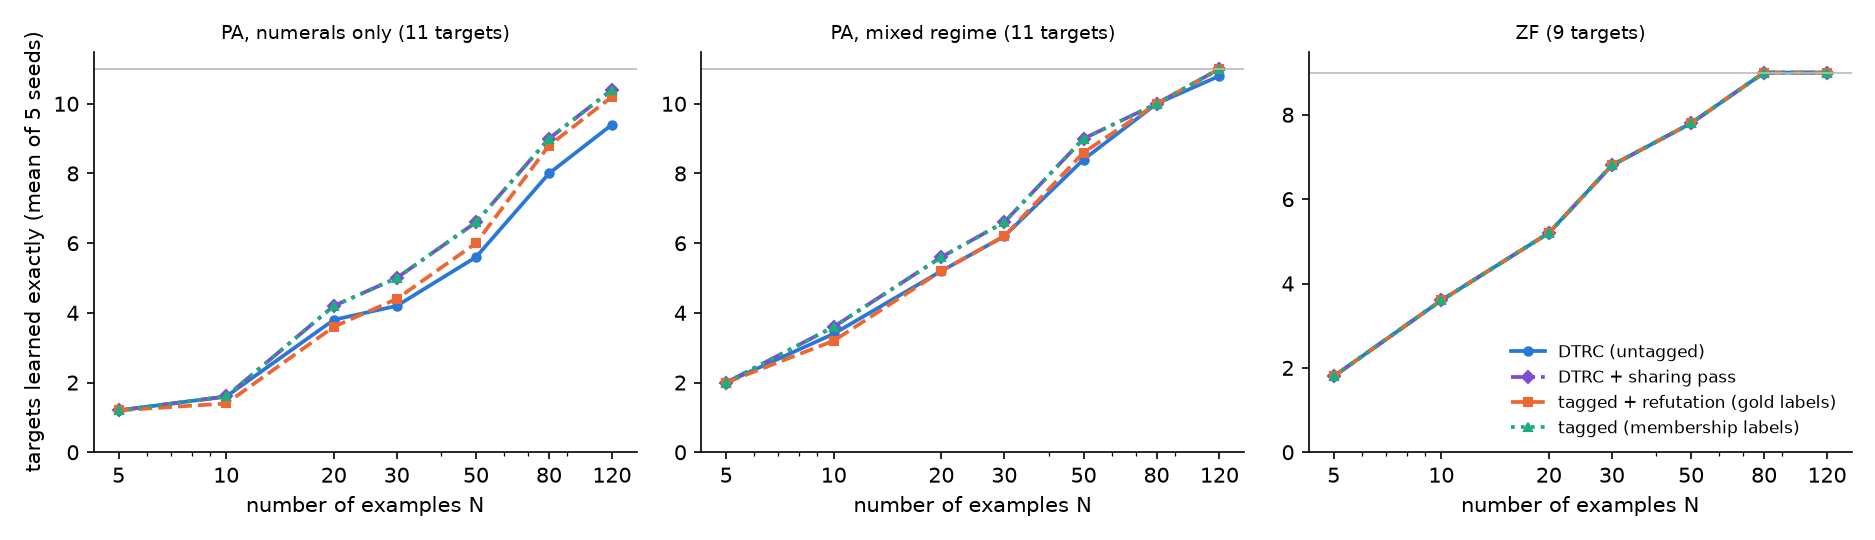
\includegraphics[width=\textwidth]{figures/e5_curves.png}
\caption{Experiment E5: number of targets learned exactly after $N$ examples (mean over seeds $0$--$4$; the rows of one stream share seeds). Left: PA, universal axioms through numerals only ($11$ targets); middle: PA, mixed regime; right: ZF ($9$ targets). \DTRC{}+share and the tagged learner with membership labels coincide; on ZF all learners coincide \src{experiments E5}.}
\label{fig:exp:e5}
\end{figure}

\paragraph{E6: the cautious $k$-union verifier without clustering.}
On $\Q$ plus induction, with no refutation negatives, $k=8$ and $k=9$ accept $0$ of $8$ held-out induction instances: one slot $\forall x\,P(x)$ covers all of $\Q$'s axioms, and each induction datum gets a singleton slot. With refutation negatives, $k=8$ accepts $8/8$ from the anchor pair alone; $k=9$ accepts $0/8$ from two induction instances (the spare slot keeps them apart) and $8/8$ from three (third motive $x+0=x$ or $\exists y\,x<y$). No false non-instance was accepted. This reproduces in $\DTF$ the prior untagged result (\cref{sec:many}) \src{experiments E6; prior pa-untagged}.

\paragraph{E7: why $\DTF$.}
Over all pairs of mixture data, $|\Min|$ in full $\DT$ exceeds $16$ for $3$ of $1176$ PA pairs (maximum $64$) and $3$ of $666$ ZF pairs (maximum $32$, with $3$ timeouts above $2$\,s, machine-dependent); in $\DTF$ the maxima are $4$ and $8$ with no timeout. This agrees with the exponential lower bound of \cref{sec:single}. Targets that need positive-arity term metavariables would need full $\DT$; the feature test of \cref{sec:single}, which avoids listing $\Min$, is not implemented \src{experiments E7, \S5}.

\paragraph{E9: refutation separation, and how narrow the evidence is.}
\Cref{tab:exp:e9} tests cross merges with the implemented refuter at budget $80$, for pairs of single data (the case to which (S) reduces) and for sets of one or two data per target; data that instantiate both targets are excluded. On the mixtures every merge is refuted. But thousands of merges reduce to $15$ (PA) and $5$ (ZF) distinct minimal templates, all refuted by $\bot$, $\forall\bar x\,\bot$, $\top\to\bot$ or a comprehension instance in the first two passes of the refuter. That is exactly what \cref{prop:exp:mixsep} proves, and it is no evidence of separation between \emph{similar} targets \src{referee F3}.

\begin{table}[t]
\centering\small
\begin{tabular}{@{}lcccc@{}}
\toprule
targets & merges tested & refuted & distinct minimal templates & distinct unrefuted\\
\midrule
PA-mix & 2200 / 2200 & 2200 / 2200 & 15 / 13 & 0 / 0\\
ZF-mix & 540 / 540 & 540 / 540 & 5 / 5 & 0 / 0\\
PA near-miss & 1080 / 1080 & 1073 / 1080 & 61 / 36 & 5 / 0\\
ZF near-miss & 225 / 225 & 225 / 225 & 5 / 5 & 0 / 0\\
ZF hard & 432 / 432 & 431 / 430 & 14 / 15 & 1 / 2\\
\bottomrule
\end{tabular}
\caption{Experiment E9: cross-target merges (pairs of single data / sets of one or two data per target), refuter budget $80$ \src{experiments E9; code/results/e9\_separation.md}.}
\label{tab:exp:e9}
\end{table}

The PA near-miss set adds $U_{\mathrm{add1}}=(z+1=Sz)$, $z\cdot1=z$, the nested $U_{\mathrm{add00}}=(z+0+0=z+0)$ and two reorderings of induction. Its unrefuted merges are valid: $n+z=S^nz$ from $n+0=n$ and $n+1=S^n1$ ($n=1,2,5,7$), and $z+0=z$ from $0+0=0$ and a $U_{\mathrm{add00}}$ datum. No world-based refuter can separate such pairs (\cref{lem:exp:valid}). The hard ZF set consists of $T_{\Sep}$, Separation from $\bigcup a$, $\ReplS$, Collection, $T_{\EInd}$, $\in$-induction along $z\in y\in x$ ($\mathrm{EInd2}$), the minimal-element schema, and the bounding forms $\mathrm{Union}_W$, $\mathrm{Power}_W$ of Union and Power taken from \cref{sec:many}.

\begin{proposition}[Two hard ZF pairs]\status{proved; computed}\src{experiments Prop E9; E9, E9b}\label{prop:exp:hard}
\textup{(a)} The unique minimal covering template of $\mathrm{Union}_W=\forall a\exists b\forall x\,(\exists y(y\in a\wedge x\in y)\to x\in b)$ and $\mathrm{Power}_W=\forall a\exists b\forall x\,(\forall y(y\in x\to y\in a)\to x\in b)$ is the universal-set schema $U=\forall a\exists b\forall x\,(P(x,a)\to x\in b)$. The ZF oracle refutes its instance $P:=\top$, although no oracle sound for $\HF\cup\{u\}$ with a universal element $u$ refutes any instance of $U$ (\cref{sec:many}).
\textup{(b)} Let $\mathrm{EInd2}(\psi)=\forall x\,(\forall y{\in}x\,\forall z{\in}y\,\psi(z)\to\psi(x))\to\forall x\,\psi(x)$. In the most frequent case (the motives' root symbols differ and the $\in$-induction motive does not begin with $\forall$), the minimal template of an $\in$-induction datum and an $\mathrm{EInd2}$ datum is $T_{EE}=(\forall x(\forall y(y\in x\to P_0(y))\to P_1(x)))\to\forall x\,P_1(x)$, which is false. Some merges of the pair are valid, and some false ones need budget $400$.
\end{proposition}

\begin{proof}[Proof idea]
(a) One clash slot ($\exists$ against $\forall$) under a common prefix. After simplification the instance is $\exists b\forall x\,(x\in b)$; with nothing concrete in scope the only case for $b$ is a fresh generic $G$, and $\forall x\,(x\in G)$ fails at $x:=G$ because $G\in G$ is false: generic objects obey Foundation. (b) $P_0:=\bot$ and $P_1(x):=\forall z\,\neg z\in x$ give the premise $\forall x\,(x=\emptyset\to x=\emptyset)$ and a conclusion that fails at $\{\emptyset\}$. Details in \cref{app:exp:stress}.
\end{proof}

The first version's oracle could not certify the premise of (b), because $\forall y\,(y\in x\to\bot)$ and $\forall z\,\neg z\in x$ were different unknown leaves; constant propagation identifies them. Ablation E9b (another $12$ random pairs): without constant propagation $0$ of $12$ merges are refuted, with it $10$ of $12$. In E9, $11$ of $12$ $\mathrm{EInd}/\mathrm{EInd2}$ pair merges were refuted; the survivor, $(\forall x(\forall y{\in}x\,\forall z{\in}y\,P_0(z,y)\to P_1(x)))\to\forall x\,P_1(x)$, is false ($P_0:=\bot$, $P_1(x):=$ ``every element of $x$ is empty'' makes the premise of the form $\alpha\to\alpha$, and the conclusion fails at $\{\{\emptyset\}\}$), and the refuter finds a refutation at budget $400$, not $80$. Valid merges also occur: $\mathrm{EInd}(x=x)$ and $\mathrm{EInd2}(x=x)$ give a template whose conclusion $\forall x\,(x=x)$ is true; and Separation and Separation from $\bigcup a$, both with body $x\in a$, give Separation with its conjuncts swapped. So (S) fails for these pairs in general \src{experiments Prop E9, E9b}.

\paragraph{E4: stress sets.}
\emph{(a) Near-miss targets} (3 seeds; PA instance schemas in the mixed regime). On ZF (adding Separation with swapped conjuncts and the minimal-element schema) the labels are recovered and all $6$ targets are exact in every seed. On PA, the three forms of induction are always separated; $U_{\mathrm{add00}}$ always merges into $U_{\mathrm{add0}}$ (nested, valid); the ambiguous numerals $0+1=1$ and $0+0=0$ join one cluster; and seed $0$ has the valid cross merges $5+z=S^5z$ and $4+z=S^4z$. Every accepted template of every mixed cluster is valid (\cref{lem:exp:valid}); $4$ probes were non-target, none refuted.

\emph{(b) Injected mistakes.} PA: $8$ mistakes (an induction-like step $\varphi(x)\to\varphi(x)$, a wrong base $\varphi(S0)$, the conclusion $\forall x\,\varphi(Sx)$, which is true but not an instance, and $n+0=0$) and $3$ true non-targets; ZF: $6$ mistakes (Separation with the comprehension variable free in the body, $\forall x(\varphi\to\varphi)\to\forall x\varphi$, complement comprehension). The clean targets stay exact: PA $11/11$ in the mixed regime and $9$--$10/11$ with numerals (the others lack an anchor), ZF $9/9$. Refuted mistakes ($2$--$3$ per run) are discarded. Unrefuted ones become singletons, each accepting itself, or merge. Every mixed cluster was examined with a post-hoc refuter (budget $4000$ for PA, $1500$ for ZF) and by hand; \cref{tab:exp:e4} in \cref{app:exp:numbers} lists the outcomes.

\begin{proposition}[A false sentence is accepted]\status{proved; computed}\src{experiments Prop E10; referee F1, R15}\label{prop:exp:qF}
In E4(b), PA-mix seed $0$, in both regimes, two mistakes (the wrong step and the $\forall x\,\varphi(Sx)$ conclusion) merge at refuter budgets $80$ and $400$ into a cluster whose only accepted template is
\[T_F=\bigl(\exists x(P_0(x,0)\wedge\neg P_1(x,0))\wedge\forall x\bigl(\exists y(P_0(y,x)\wedge\neg P_1(y,x))\to\exists y(y<Sx\wedge\neg P_1(y,Sx))\bigr)\bigr)\to\forall x\,\exists y\,(y<Sx\wedge\neg P_1(y,Sx)).\]
With $P_0(y,x):=(x=0)$ and $P_1(y,z):=(z=2)$ it has the instance
\[q_F=\bigl(\exists x(0=0\wedge\neg\,0=2)\wedge\forall x\bigl(\exists y(x=0\wedge\neg\,x=2)\to\exists y(y<Sx\wedge\neg\,Sx=2)\bigr)\bigr)\to\forall x\,\exists y\,(y<Sx\wedge\neg\,Sx=2),\]
which is false in $\N$ and an instance of no PA-mix target. \DTRC{} accepts $q_F$ at budgets $80$ and $400$, and not at budget $2000$.
\end{proposition}

\begin{proof}
The first premise is true. The second is true: at $x=0$ the consequent holds with $y=0$, since $1\neq2$; at $x\ge1$ the antecedent is false. The conclusion fails at $x=1$, where $Sx=2$. The rest is computed (E4(b), recheck R15).
\end{proof}

Refuting $q_F$ needs a certificate for the $\Pi_1$ second premise, i.e.\ a case split on $x=0$. The first version's oracle returns unknown on $q_F$; the revised oracle returns False, but the refuter does not reach this instance within $80$ or $400$ tries. The probes of E4 never sampled $q_F$ and reported ``$0$ refuted'' in every row, including the rows where $q_F$ is accepted. The first version of the record claimed that PA mistakes merge only into valid templates; the referee found this exhibit, and the claim is withdrawn. Two lessons: \emph{with mistakes in the data, \DTRC{}'s union is not truth-sound even in arithmetic}, and \emph{probe counts are lower bounds on unsoundness}.

The other residual merges are valid:

\begin{lemma}[Validity of the residual templates]\status{proved}\src{experiments Lemma V}\label{lem:exp:valid}
Every instance of each of the following templates is true in $\N$ (items 1--4) or in $V$ (item 5).
(1)~$S^n0+z=S^nz$, $n\ge0$.
(2)~$z+1=Sz$, $z+0=z$, $0+z=z$.
(3)~Templates of the form $(\alpha\wedge\dots)\to\dots$ whose first antecedent conjunct $\alpha$ is $z<0$, $0=Sz$, or $\exists x(x<t\wedge\dots)$ with $t\in\{0,\ 0+0,\ 0\cdot0\}$.
(4)~$(P(0)\wedge\forall x(P(x)\to P(Sx)))\to\forall x\,P(Sx)$.
(5)~$\forall x\,(P(x)\to x=x)\to\forall x\,(x=x)$ and $\forall x\,(\forall y(y\in x\to P(y))\to x=x)\to\forall x\,(x=x)$.
\end{lemma}

\begin{proof}
(1) $n+t=S^n(t)$ in $\N$. (2) These are true instance schemas. (3) The conjunct $\alpha$ is false in $\N$. (4) By induction $\forall x\,P(x)$, hence $\forall x\,P(Sx)$. (5) The conclusion is true.
\end{proof}

The false templates met in E4(b) are $T_F$ (budgets $80$ and $400$), two induction-step templates in the numerals regime at budget $80$, and five Separation-capture templates on ZF at budget $80$; each has a hand-checked false instance (\cref{app:exp:stress}). At budget $400$ no false ZF merge remains, and at budget $2000$ no false PA merge remains. The cost grows with the budget: PA $714$--$1217$ oracle calls at budget $80$, $1624$--$3848$ at $400$, $3048$--$10684$ at $2000$; ZF $795$--$874$ at $80$, $2004$--$2445$ at $400$ \src{experiments E4}.

\emph{(c) Unequal frequencies} (PA: induction $60$, $U_{\mathrm{add0}}$ $20$, $U_{\mathrm{mul0}}$ $3$, $U_{\mathrm{0add}}$ $1$, numerals only; ZF: Separation $30$, Replacement $4$, $\in$-induction $1$; 3 seeds). Frequent targets are exact (induction and Separation $3/3$; $U_{\mathrm{add0}}$ $1/3$ for \DTRC{} and $2/3$ with sharing, since $0+0=0$ is its only anchor); Replacement and $U_{\mathrm{mul0}}$ are exact in $2/3$. Targets with one instance are never generalized ($0/30$ held-out $\in$-induction instances, $0/20$ for $U_{\mathrm{0add}}$). No non-target probe.

% ---------------------------------------------------------------------
\subsection{Limitations}\label{sec:exp:limits}

\begin{enumerate}
\item \emph{Budgeted refutation accepts false sentences.} A merge whose minimal templates are false, but whose false instances the refuter does not reach, makes \DTRC{} accept false sentences (\cref{prop:exp:qF}). The search order and pools are heuristic; the $\top/\bot$ and one-at-a-time passes and the PA case split fix the cases met here at budget $400$ (ZF) or $2000$ (PA). Whether some natural refuter refutes every false minimal template of a cross pair of mixture data within a budget polynomial in the data size is open.
\item \emph{Valid residual merges} cannot be separated by any world-based method, since the merged set is true: $n+z=S^nz$, nested targets, templates with a false antecedent or a true conclusion, some $\mathrm{EInd}/\mathrm{EInd2}$ and Separation pairs. \DTRC{} is then truth-sound but not target-sound (\cref{sec:many}).
\item \emph{Ambiguous data.} A datum in two instance sets goes to one cluster under a partition, and can cost the other target its only anchor. The sharing pass repairs this under (S$^+$) and (P); a guarantee without (P), e.g.\ when the singleton $\{0+0=0\}$ is a final cluster, is open.
\item \emph{Oracle limits.} No witness is constructed from generics or terms (\cref{sec:exp:impl}); extending the generics by constructions such as $\{G\}$ or $G\cup\{c\}$ would refute comprehension failures such as $\forall a\exists b\forall x\,(x\in b\leftrightarrow a\in x)$.
\item \emph{Singletons.} A target with one instance is never generalized, and an unrefuted mistake becomes a singleton that the union accepts; without labels or frequencies it cannot be told from a ground axiom.
\item \emph{The class.} $\DTF$ excludes positive-arity term metavariables (E7).
\item \emph{Greedy order.} Without (S) the final partition can depend on the merge order, and there is no theorem for that case; the sharing pass is greedy in data order.
\item \emph{Evidence for separation} is a proof for the mixture targets (\cref{prop:exp:mixsep}) and little more. Characterizing, in terms of the targets alone, when two targets admit only refutable cross merges is open; the observed failures are a false antecedent, a true conclusion, an instance shared with a third target, and nesting.
\item \emph{Scale.} The code is pure Python; the ZF oracle dominates the running time (the largest single run took $13$\,s; all experiments take about $10$ minutes).
\end{enumerate}
